% !TeX program = pdflatex
\documentclass{iutbscthesis}
\usepackage{amsmath}
\usepackage{amssymb}
  % for mathematical symbols
\addbibresource{citations.bib}

\title{Reinforcement Learning with Verifiable Rewards for Chart Question Answering}

\addauthor{Sumaiya Ahmed}{210041223}
\addauthor{Nafisa Haque}{210041231}
\addauthor{Jannatul Fardus Rakhi}{210041237}

\supervisor{Syed Rifat Raiyan}{Lecturer}{Department of Computer Science and Engineering}

\addcosupervisor{Dr.\ Hasan Mahmud}{Professor}{Department of Computer Science and Engineering}
\addcosupervisor{Dr.\ Md.\ Kamrul Hasan}{Professor}{Department of Computer Science and Engineering}

\department{Department of Computer Science and Engineering}
\program{BACHELOR OF SCIENCE IN COMPUTER SCIENCE AND ENGINEERING}
\defensedate{22}{April}{2026}

\begin{document}

%-------------------------- FRONT MATTER --------------------------%

\coverpage
\pagenumbering{roman}
\declarationofcandidate

\dedicatedto{our supervisors, for their guidance at every stage of this work}

\tableofcontents
\listoffigures
\listoftables

\clearpage

\begin{abbreviations}
    \abbr{CoT}{Chain-of-Thought}
    \abbr{CQA}{Chart Question Answering}
    \abbr{GRPO}{Group Relative Policy Optimization}
    \abbr{HCPC}{Hierarchical Correct-Path Consistency}
    \abbr{KL}{Kullback-Leibler}
    \abbr{LoRA}{Low-Rank Adaptation}
    \abbr{NSR}{Negative Sample Reward}
    \abbr{OOD}{Out-of-Distribution}
    \abbr{QA}{Question Answering}
    \abbr{RL}{Reinforcement Learning}
    \abbr{RLVR}{Reinforcement Learning with Verifiable Rewards}
    \abbr{SFT}{Supervised Fine-Tuning}
    \abbr{VLM}{Vision-Language Model}
    \abbr{VQA}{Visual Question Answering}
\end{abbreviations}

\begin{acknowledgement}
We are grateful to our supervisor, Syed Rifat Raiyan, whose direction kept this project grounded from its earliest conceptual stages through the final evaluation runs. His willingness to engage with the technical details of reward design and his patience when training results raised more questions than they answered made a genuine difference to the quality of this work.

We thank Dr.\ Hasan Mahmud and Dr.\ Md.\ Kamrul Hasan for their guidance on evaluation methodology and for consistently pushing us to think carefully about what the numbers actually mean, not just whether they were large.

We are also grateful to the Systems and Software Lab for providing the computational resources and collaborative environment that made this research possible.

Finally, we thank our families for their patience through months of training runs, late-night debugging sessions, and the particular kind of stress that comes from watching a long GPU job fail near completion.
\end{acknowledgement}

\begin{abstract}
Chart question answering requires a model to answer natural language questions directly from chart images, without manual data annotation or chart-specific templates. Current vision-language models trained with supervised fine-tuning are brittle under distribution shift and frequently produce reasoning traces that are not grounded in the chart's actual values. This thesis proposes HCPC-RLVR, a reinforcement learning with verifiable rewards framework that fine-tunes Qwen2.5-VL-3B-Instruct on 1,000 chart-question training samples using Group Relative Policy Optimization. The primary contribution is the Hierarchical Correct-Path Consistency reward, a cross-rollout bonus conditioned on intermediate correctness that encourages stable table extraction and diverse reasoning among rollouts that are fully correct. As a competitive baseline, Negative Sample Reward is applied to a vision-language model for the first time, extending negative-only reinforcement from text-based mathematics to a multi-modal setting with noisy, multi-component rewards.

Evaluation on the 500-sample Chart-RVR GRPO Test 151 split shows that every RLVR-trained variant substantially outperforms the untrained base model. The base model obtains 59.45\% Pass@1 and 84.46\% Pass@4. GRPO improves this to 73.0\% Pass@1 and 87.31\% Pass@4. GRPO+HCPC obtains the strongest four-rollout behavior, with the highest Pass@2 (84.57\%) and Pass@4 (88.70\%). NSR obtains the strongest Pass@1 (73.4\%) and remains close at Pass@4 (88.00\%). Out-of-distribution evaluation on 500 ChartFC samples shows NSR as the strongest method across Pass@K: NSR reaches 68.70\% Pass@1 and 92.40\% Pass@4, compared with 61.22\% and 83.14\% for GRPO+HCPC, and 62.45\% and 81.8\% for GRPO. These findings indicate that reward design, particularly whether the training signal preserves diversity and conditions on intermediate reasoning steps, is a meaningful lever for improving structured visual reasoning in small-scale vision-language models.
\end{abstract}

%-------------------------- MAIN BODY --------------------------%
\pagenumbering{arabic}

\chapter{Introduction}

The modern information landscape is increasingly mediated through visual representations of data. Charts, plots, and statistical figures have become the dominant medium through which quantitative findings are communicated across scientific literature, financial reporting, and public policy \cite{masry2022chartqa}. As datasets grow in scale and complexity, visual encodings have emerged as the preferred abstraction for conveying structured relationships, making the automatic parsing and reasoning over chart images an important research problem at the confluence of computer vision, natural language processing, and structured reasoning. 
\\
Chart Question Answering (Chart QA) formalizes this capacity as the problem of generating correct natural language answers to questions posed over chart images \cite{masry2022chartqa, masry2024chartinstruct}. The task is deceptively complex. Unlike generic visual question answering, Chart QA imposes a strict sequential dependency across multiple reasoning stages: a model must first recognize the chart type, reconstruct the underlying data with sufficient precision, and only then apply the appropriate numerical or logical operation to produce a verifiable answer. Each stage introduces its own failure mode, and errors propagate  an incorrectly identified chart type corrupts the extraction strategy, and an imprecise data table renders any downstream computation unreliable. This layered structure makes Chart QA a particularly demanding testbed for evaluating the reasoning depth of vision-language models (VLMs). \\
Progress in this area has accelerated with the development of large multimodal models. Architectures such as Qwen2.5-VL \cite{qwen25vl}, Gemma3 \cite{gemma3}, and InternVL \cite{internvl} couple high-capacity visual encoders with transformer-based language model backbones, \\ achieving  competitive 
accuracy on standard benchmarks such as ChartQA \cite{masry2022chartqa} and PlotQA \cite{plotqa}. However, benchmark performance masks two persistent failure modes that significantly limit the practical utility of current approaches. \\
The first is \textit{reasoning collapse}. When trained with standard reinforcement learning objectives specifically Group Relative Policy Optimization (GRPO) \cite{shao2024deepseekmath}  models are strongly reinforced toward whichever single reasoning strategy yields correct answers during training, suppressing alternative valid paths. The consequence is severe: Chart-RVR \cite{sinha2025chartrvr}, the current state-of-the-art framework, achieves 84.6 percent accuracy on in-domain ChartQA samples yet drops to 53.4 percent  on EvoChart \cite{chartx2024}, an out-of-distribution benchmark  a gap exceeding 31 percentage points that reflects the diversity-suppressing gradient dynamics of standard policy optimization. \\
The second is \textit{hallucinated reasoning}. Standard reward formulations condition solely on the correctness of the final answer, without verifying whether intermediate reasoning steps are consistent with the model's own extracted data. This creates a critical loophole: a model can receive full reward for a response in which the reasoning trace references values entirely absent from the extracted table \cite{wen2025rlvr}. Such models are epistemically unreliable their apparent correctness on familiar inputs provides no assurance of faithfulness on novel ones.
Together, these two failure modes the collapse of reasoning diversity under standard policy optimization, and the tolerance of hallucinated intermediate steps under answer-only reward signals constitute the central limitations that motivate the present work.

\section{Task Definition}

Let $\mathcal{I}$ denote a chart image and $\mathcal{Q}$ a natural language question posed over that image. The Chart Question Answering task requires learning a mapping:

\begin{equation}
    M(\mathcal{I}, \mathcal{Q}) \rightarrow (\mathcal{R}, \mathcal{A})
\end{equation}

\noindent where $\mathcal{R} = \{r_1, r_2, \ldots, r_t\}$ is a structured reasoning chain and $\mathcal{A}$ is the final answer. A response is valid if and only if $\mathcal{A}$ is correct with respect to the ground truth and every step $r_i \in \mathcal{R}$ is grounded in values extracted directly from $\mathcal{I}$.

The reasoning chain $\mathcal{R}$ follows a hierarchical structure across four levels:

\begin{enumerate}
    \item \textbf{Perception:} Identify the chart type $\tau \in \{\text{bar, line, pie, stacked bar, ...}\}$ from the visual structure of $\mathcal{I}$.
    \item \textbf{Extraction:} Parse the chart into a structured data table $\mathcal{T} = \{(k_j, v_j)\}_{j=1}^{n}$, where $k_j$ and $v_j$ denote the label and numerical value of the $j$-th data point respectively.
    \item \textbf{Reasoning:} Apply numerical or logical operations over $\mathcal{T}$ to derive an intermediate result supporting the final answer.
    \item \textbf{Answer:} Produce the final response $\mathcal{A}$ consistent with the reasoning step.
\end{enumerate}

The perception and extraction levels admit a single correct outcome and therefore demand \textit{consistency} across model outputs. The reasoning level, however, admits multiple valid strategies, such as summation, comparison, or percentage computation, and therefore benefits from \textit{diversity}. A model capable of multiple reasoning strategies generalizes more robustly to unseen chart distributions.

Formally, a fully correct rollout is defined as:

\begin{equation}
    \mathcal{F} = \left\{ r \in \mathcal{R} \;\middle|\; \tau_r = \tau^*, \quad \text{sim}(\mathcal{T}_r, \mathcal{T}^*) \geq \delta, \quad \mathcal{A}_r = \mathcal{A}^* \right\}
\end{equation}

\noindent where $\tau^*$, $\mathcal{T}^*$, and $\mathcal{A}^*$ denote the ground-truth chart type, data table, and answer respectively, $\text{sim}(\cdot,\cdot)$ is a table similarity function, and $\delta = 0.8$ is the acceptance threshold. This formulation distinguishes the present work from prior approaches that condition rewards solely on $\mathcal{A}$, ignoring whether $\mathcal{R}$ is faithful to $\mathcal{T}$, and directly motivates the hierarchical reward design .

\section{Background}

\subsection{Reinforcement Learning}

Reinforcement learning (RL) concerns an agent learning a policy $\pi_\theta$ by interacting
with an environment to maximise expected cumulative reward. At each timestep $t$, the
agent observes a state $s_t$, selects an action $a_t \sim \pi_\theta(\cdot \mid s_t)$, and receives a scalar
reward $r_t$. The objective is to find parameters $\theta$ that maximise the expected return:

\begin{equation}
    J(\theta) = \mathbb{E}_{\tau \sim \pi_\theta}\!\left[\sum_{t=0}^{T} \gamma^t r_t\right]
\end{equation}

\noindent where $\tau = (s_0, a_0, r_0, \ldots, s_T)$ is a trajectory sampled under $\pi_\theta$ and
$\gamma \in (0,1]$ is a discount factor that controls the relative importance of future rewards.

In the language model setting, the agent is the model itself, the state at step $t$ is the
concatenation of the input prompt $x$ and all tokens generated so far, and each action
is the selection of the next token from the model's vocabulary. A complete generated
sequence $y = (a_0, a_1, \ldots, a_T)$ is referred to as a \textit{rollout}. The reward $r(y, y^*)$
is assigned to the rollout as a whole after generation completes, where $y^*$ denotes the
ground-truth reference.

Policy optimisation proceeds via the policy gradient theorem \cite{sutton1999policy}.
The gradient of the objective with respect to $\theta$ is:

\begin{equation}
    \nabla_\theta J(\theta) = \mathbb{E}_{\tau \sim \pi_\theta}\!\left[
        \sum_{t=0}^{T} \nabla_\theta \log \pi_\theta(a_t \mid s_t)\, A_t
    \right]
\end{equation}

\noindent where $A_t$ is the \textit{advantage} at timestep $t$, measuring how much better action
$a_t$ is relative to the expected value of the current policy from state $s_t$:

\begin{equation}
    A_t = \sum_{t'=t}^{T} \gamma^{t'-t} r_{t'} - V(s_t)
\end{equation}

\noindent Here $V(s_t)$ is a baseline value function that reduces gradient variance without
introducing bias. The simplest instantiation, REINFORCE \cite{williams1992simple},
uses the empirical return as the advantage estimate and performs a single gradient step
per rollout:

\begin{equation}
    \nabla_\theta J(\theta) \approx \frac{1}{K}\sum_{i=1}^{K}
        \sum_{t=0}^{T} \nabla_\theta \log \pi_\theta(a_t^{(i)} \mid s_t^{(i)})\, \hat{A}_t^{(i)}
\end{equation}

\noindent where $K$ rollouts are sampled to reduce estimator variance.

\subsection{Policy Optimisation in Deep Reinforcement Learning}

Naive policy gradient methods suffer from high variance and sensitivity to step size:
a large update can collapse the policy into a degenerate distribution from which
recovery is difficult. Proximal Policy Optimisation (PPO) \cite{schulman2017proximal}
addresses this by constraining each update so that the updated policy $\pi_\theta$ does not
deviate excessively from the previous policy $\pi_{\theta_{\text{old}}}$. PPO maximises a clipped
surrogate objective:

\begin{equation}
    \mathcal{L}^{\text{CLIP}}(\theta) = \mathbb{E}_t\!\left[
        \min\!\left(
            \rho_t(\theta)\, A_t,\;
            \text{clip}\!\left(\rho_t(\theta),\, 1{-}\epsilon,\, 1{+}\epsilon\right) A_t
        \right)
    \right]
\end{equation}

\noindent where $\rho_t(\theta) = \pi_\theta(a_t \mid s_t) / \pi_{\theta_{\text{old}}}(a_t \mid s_t)$ is the
probability ratio between the updated and reference policies, and $\epsilon$ is a small
hyperparameter (typically $0.1$--$0.2$) that defines the trust region. The clipping
prevents the ratio from moving outside $[1{-}\epsilon,\, 1{+}\epsilon]$, bounding the policy
shift at each update.

An alternative mechanism for constraining policy updates is the KL divergence
penalty, which augments the reward with a term that penalises deviation from a
reference policy $\pi_{\text{ref}}$:

\begin{equation}
    \tilde{r}_t = r_t - \beta\, \mathbb{D}_{\text{KL}}\!\left[\pi_\theta(\cdot \mid s_t)
        \;\|\; \pi_{\text{ref}}(\cdot \mid s_t)\right]
\end{equation}

\noindent where $\beta > 0$ controls the strength of the penalty. In language model fine-tuning,
$\pi_{\text{ref}}$ is typically the supervised pre-trained checkpoint, ensuring that RL training
does not degrade the model's general language capabilities while optimising for
task-specific reward. This penalty is employed in several RLVR frameworks and
serves as a regulariser against reward hacking.

\subsection{Reinforcement Learning with Verifiable Rewards}

Standard RL for language models often relies on a learned reward model trained on
human preference annotations \cite{ouyang2022training}. Such reward models introduce
a second source of approximation error and are susceptible to reward hacking — the
policy learns to exploit weaknesses in the reward model rather than genuinely solving
the task. Reinforcement Learning with Verifiable Rewards (RLVR)
\cite{lightman2023lets} eliminates this vulnerability by restricting the reward signal
to objective, rule-based criteria. A reward is assigned only when the model's output
satisfies a deterministic ground-truth check:

\begin{equation}
    r(y, y^*) = \begin{cases}
        1 & \text{if } \texttt{verify}(y,\, y^*) = \texttt{True} \\
        0 & \text{otherwise}
    \end{cases}
\end{equation}

\noindent where \texttt{verify} is a domain-specific correctness function. For mathematical
reasoning, this function checks numerical equivalence; for chart question answering,
it checks whether the extracted answer matches the annotated ground truth within a
specified tolerance.

The policy gradient under RLVR is obtained by substituting this binary reward into
the standard update rule. Because rewards are sparse most rollouts receive zero
reward variance reduction is critical. Sampling $K$ rollouts per input and computing
group-relative advantages (see Section~\ref{sec:policy_strategies}) is the standard
approach. RLVR has demonstrated strong results on mathematical reasoning
\cite{shao2024deepseekmath} and has more recently been extended to visual reasoning
domains \cite{yang2025r1v}, motivating its application to chart question answering
in this work.

\subsection{Policy Update Strategies}
\label{sec:policy_strategies}

Three policy update strategies are relevant to this work. All three share the same
group-sampling procedure: given an input $x$, $K$ rollouts
$\{y_1, \ldots, y_K\}$ are sampled from the current policy and each is scored by the
verifiable reward $r_i = r(y_i, y^*)$.

\subsubsection{Group Relative Policy Optimisation}

Group Relative Policy Optimisation (GRPO) \cite{shao2024deepseekmath} replaces the
value network of PPO with a group-mean baseline. The advantage of rollout $i$ is:

\begin{equation}
    A_i^{\text{GRPO}} = \frac{r_i - \mu_r}{\sigma_r + \varepsilon},
    \quad \mu_r = \frac{1}{K}\sum_{j=1}^K r_j,
    \quad \sigma_r = \sqrt{\frac{1}{K}\sum_{j=1}^K (r_j - \mu_r)^2}
\end{equation}

\noindent where $\varepsilon$ is a small constant for numerical stability. The policy is updated
by maximising the clipped surrogate objective with a KL penalty:

\begin{equation}
    \mathcal{L}^{\text{GRPO}}(\theta) = \mathbb{E}\!\left[
        \frac{1}{K}\sum_{i=1}^{K}\min\!\left(
            \rho_i A_i^{\text{GRPO}},\;
            \text{clip}(\rho_i, 1{-}\epsilon, 1{+}\epsilon)\, A_i^{\text{GRPO}}
        \right)
    \right] - \beta\, \mathbb{D}_{\text{KL}}[\pi_\theta \| \pi_{\text{ref}}]
\end{equation}

\noindent where $\rho_i = \pi_\theta(y_i \mid x) / \pi_{\theta_{\text{old}}}(y_i \mid x)$.
GRPO is computationally efficient and eliminates the need for a separate critic
network. However, its strong reinforcement of above-average rollouts can concentrate
probability mass on a single dominant reasoning template — a phenomenon termed
\textit{reasoning collapse} — reducing the model's ability to generalise to
out-of-distribution inputs.

\subsubsection{Negative Sample Reward}

Negative Sample Reward (NSR) \cite{yu2025dapo} addresses reasoning collapse by
treating correct and incorrect rollouts asymmetrically. Correct rollouts receive a zero
gradient update, while incorrect rollouts receive a negative update:

\begin{equation}
    A_i^{\text{NSR}} = \begin{cases}
        0   & \text{if } r_i = 1 \\
        -1  & \text{if } r_i = 0
    \end{cases}
\end{equation}

The corresponding policy update penalises incorrect rollouts without reinforcing any
particular correct path:

\begin{equation}
    \mathcal{L}^{\text{NSR}}(\theta) = \mathbb{E}\!\left[
        \frac{1}{K}\sum_{i=1}^{K} \mathbf{1}[r_i = 0]\,
        \nabla_\theta \log \pi_\theta(y_i \mid x)
    \right]
\end{equation}

The intuition is that reinforcing correct rollouts concentrates probability mass on a
single solution template, whereas penalising only incorrect rollouts allows the model
to maintain multiple valid reasoning strategies simultaneously, thereby preserving
output diversity.

\subsubsection{Weighted REINFORCE}

Weighted REINFORCE (W-REINFORCE) \cite{yu2025dapo} adopts a hybrid position
between GRPO and NSR. Correct rollouts receive a weak positive update scaled by a
coefficient $\lambda \ll 1$, while incorrect rollouts receive a full negative update:

\begin{equation}
    A_i^{\text{W-REINFORCE}} = \begin{cases}
        \lambda  & \text{if } r_i = 1 \\
        -1       & \text{if } r_i = 0
    \end{cases}
\end{equation}

\noindent With $\lambda = 0.1$, the update provides a gentle positive signal for correct
rollouts while still strongly suppressing incorrect ones. This asymmetry attempts to
balance answer accuracy with diversity preservation, avoiding the distribution collapse
of GRPO while retaining some reinforcement signal for correct behaviour. In this
work, W-REINFORCE is discussed as background context; the primary experimental
comparison focuses on GRPO, GRPO with the proposed HCPC reward, and NSR.

\section{Research Objectives}

The objectives of this thesis are as follows:

\begin{enumerate}
    \item Fine-tune Qwen2.5-VL for chart question answering via RLVR under realistic resource constraints.
    \item Test whether reward shaping can improve chart QA without relying on large supervised demonstration corpora.
    \item Introduce the HCPC reward for consistent table extraction and diverse reasoning across rollouts.
    \item Compare explicit diversity promotion through HCPC with implicit diversity preservation through NSR.
    \item Measure not only final-answer accuracy, but also rollout reliability, table consistency, reasoning diversity, coherence, and format compliance.
    \item Analyze where current reward designs fail, especially on line charts, decimal precision, color grounding, and out-of-distribution fact-checking inputs.
\end{enumerate}

\section{Research Challenges}

Applying RLVR to chart question answering is harder than applying it to text-only reasoning tasks, for reasons that go beyond the addition of visual input.

\textbf{Reasoning collapse and hallucination.} Existing RLVR methods trained with positive reinforcement alone tend to converge toward a small set of dominant reasoning patterns \cite{sinha2025chartrvr, wen2025rlvr}. In the chart setting this is particularly damaging because a collapsed strategy often works for common chart layouts but fails on out-of-distribution inputs. Hallucination citing numeric values in the reasoning chain that do not appear in the chart is a related problem that correct-answer rewards alone cannot detect.

\textbf{Inadequate evaluation metrics.} Standard metrics like Pass@K reward correct final answers regardless of whether the intermediate reasoning is valid \cite{wen2025rlvr, zhu2025rlvrdecomposed}. This can make RLVR appear less effective than it actually is, since base models sometimes guess correct answers through entirely incorrect reasoning, artificially inflating their apparent performance.

\textbf{Output diversity destruction.} Positive reinforcement systematically collapses output diversity \cite{zhu2025rlvrdecomposed, sinha2025chartrvr}. For tasks where multiple valid reasoning paths exist --- as in chart QA, where the same answer can often be reached by reading different subsets of the data table --- this is a significant practical limitation when the goal is a robust system rather than one that performs well on average.

\textbf{Flat reward design.} Existing reward frameworks treat all reasoning levels uniformly, assigning the same signal regardless of whether a model correctly identifies the chart type, accurately reconstructs the data table, or produces a correct final answer \cite{sinha2025chartrvr}. A flat reward cannot distinguish between a model that arrives at the right answer through correct intermediate steps and one that hallucinated the intermediate steps but happened to get the final answer right.

\section{Research Questions}

This thesis is organized around seven research questions.

\begin{enumerate}
    \item Can RLVR, with only 1,000 training samples and a 3B-parameter VLM, produce meaningful improvements in chart QA accuracy and output structure?
    \item Does a hierarchical reward (HCPC) that conditions bonuses on intermediate reasoning correctness outperform flat GRPO rewards?
    \item Does HCPC simultaneously promote reasoning diversity across rollouts and maintain extraction consistency?
    \item Can NSR, designed for text-only mathematical reasoning, transfer to a vision-language model with multi-component, noisy rewards?
    \item How do different reward strategies affect out-of-distribution generalization?
    \item What is the empirical relationship between table extraction consistency, reasoning diversity, and answer correctness?
    \item How does explicit diversity promotion (HCPC) compare to implicit diversity promotion (NSR) in terms of accuracy, rollout reliability, and reasoning quality?
\end{enumerate}

\section{Contributions}

The specific contributions of this thesis are:

\begin{itemize}
    \item \textbf{HCPC reward:} A cross-rollout bonus that rewards consistent table extraction and diverse reasoning among fully-correct rollouts, conditioning the reward on intermediate step correctness rather than the final answer alone.
    \item \textbf{First VLM application of NSR:} Negative Sample Reward extended from text-only mathematics to a multi-modal model with noisy, multi-component rewards.
    \item \textbf{Empirical comparison of reward strategies:} Systematic evaluation of GRPO, GRPO+HCPC, and NSR on 500 in-distribution Chart-RVR GRPO Test 151 samples and 500 out-of-distribution ChartFC samples, reporting Pass@K for $K \in \{1, 2, 4\}$.
    \item \textbf{Resource-aware experimental analysis:} A clear separation between the intended $K=8$ HCPC design and the current $K=4$ experimental setting used because of compute constraints.
\end{itemize}

\section{Organization}
Surveys related work on chart understanding benchmarks, supervised fine-tuning, reinforcement learning for reasoning, and structured chain-of-thought methods. Chapter~\ref{chapter:proposed} describes the proposed methodology, including reward components, policy update rules, and training configuration. Chapter~\ref{chapter:results} presents the experimental setup and results on the in-distribution Chart-RVR test split and the out-of-distribution ChartFC benchmark. Chapter~\ref{chapter:conclusion} summarizes the findings, discusses limitations, and outlines directions for future work.

\section{Why Charts Are a Distinct Visual Reasoning Problem}

Chart images differ from natural images in a way that is important for model design. In natural-image visual question answering, many questions can be answered by recognizing objects or scenes: whether a dog is present, what color a car is, or how many people appear in the frame. The relevant evidence is usually spatially localized and semantically familiar. A chart image, by contrast, is an encoded representation of a table. The visible marks are not the answer by themselves; they must be decoded through conventions such as axes, legends, tick intervals, colors, bar heights, line slopes, and slice angles. A model that recognizes that an image is a bar chart has only solved the first part of the problem. It must still reconstruct the values represented by the bars and connect those values to the wording of the question.

This makes chart QA naturally hierarchical. At the lowest level, the model must parse visual marks into data values. At the next level, it must associate those values with labels and units. At the reasoning level, it must perform operations such as comparison, addition, subtraction, ratio calculation, or temporal trend identification. Finally, it must express the answer in the expected format. Errors at these levels are not independent. If the extracted table is wrong, the final answer may still accidentally match the ground truth, but the reasoning path is not reliable. If the table is correct but the arithmetic is wrong, perception succeeded but reasoning failed. If the answer is correct but the output tags are malformed, the response may be unusable for downstream automated evaluation. This thesis therefore treats chart QA as a structured reasoning pipeline rather than a single answer-generation task.

\section{Motivation for Verifiable Rewards}

Supervised fine-tuning teaches a model to imitate target responses. This is useful when the response style is important, but it does not directly answer whether the generated reasoning is correct. In chart QA, a supervised target often contains a particular chain of thought even though multiple chains could be valid. For example, a question asking for the difference between two values can be solved by subtracting the smaller value from the larger value directly, by computing both values from percentages, or by first converting units and then subtracting. A model trained only to imitate one demonstration may be penalized for a different but valid route, while a model trained with verifiable rewards can be evaluated on whether its output satisfies objective checks.

RLVR is attractive here because chart QA has several verifiable substructures. The chart type can be checked against a label. The extracted table can be compared against a ground-truth table. The final answer can be checked with relaxed numeric matching. The response format can be checked with a parser. These checks are not perfect, but they are objective and cheap compared with human preference annotation. The main design challenge is how to combine them into a reward that improves reasoning rather than merely improving answer guessing. HCPC addresses this challenge by applying an additional reward only to the subset of rollouts that are correct through the intermediate path, not merely correct at the final answer.

\section{Scope of the Present Work}

This thesis focuses on training-time reinforcement learning for a single 3B-parameter vision-language model. It does not introduce a new chart parser, a new benchmark, or a multi-agent inference system. The choice is deliberate: the goal is to isolate the effect of reward design under constrained compute. A system with external tools, symbolic solvers, or larger models may achieve higher absolute accuracy, but it would make it harder to determine whether the reward strategy itself improved the model's visual reasoning behavior.

The proposed HCPC design is naturally defined over $K=8$ rollouts, because diversity and consistency are group-level properties that become more reliable when estimated from more samples. The current experiments use four generated responses per sample due to resource constraints in training and evaluation. This means that the reported results should be interpreted as an initial resource-constrained validation of the method rather than the full intended $K=8$ setting. Extending the experiments to $K=8$ is therefore not a change in the method, but the natural next stage of completing the intended design.


\section{Related Work}

\subsection{Chart Question Answering Benchmarks}

The ChartQA benchmark \cite{masry2022chartqa} established the standard evaluation
protocol for chart question answering, providing question-answer pairs over diverse
chart types and separating evaluation into perception subtasks, which require reading
a value directly from the chart, and reasoning subtasks, which require computation
over multiple extracted values. This separation is significant because it isolates the
two failure modes that a capable system must address independently: visual
misperception and reasoning error. ChartQA adopts a relaxed correctness criterion
that tolerates numeric near-matches, acknowledging that pixel-level ambiguity in
axis reading means that slightly different extracted values may all be defensible.
This thesis uses ChartQA as the primary evaluation benchmark alongside ChartFC
\cite{akhtar2023chartfc}, which extends chart understanding to fact-checking, requiring
models to verify whether a textual claim is supported or refuted by a given chart.

\subsection{Supervised Fine-Tuning for Chart Reasoning}

Prior to reinforcement learning approaches, supervised fine-tuning on chart-specific
instruction datasets was the dominant paradigm. ChartInstruct \cite{liu2024chartinstruct}
fine-tuned a vision-language model on large-scale chart instruction data, while
ChartGemma \cite{masry2024chartgemma} applied visual instruction tuning across
diverse chart types. Carbune et al. \cite{carbune2024chart} demonstrated that
reasoning capability could be distilled from text-only chain-of-thought data into
smaller VLMs without large-scale chart-specific annotation.

The fundamental limitation of SFT-based approaches is brittleness under
distribution shift. When test charts differ in visual style, axis conventions, or
topic from training charts, performance degrades because the model learns to
match demonstrations rather than construct grounded reasoning from the chart
it receives \cite{onoe2024chartrvr}. This limitation is the primary motivation for
adopting reinforcement learning, whose training signal depends on outcome
correctness rather than similarity to demonstrations.

\subsection{Reinforcement Learning for Chart Reasoning}

The Chart-RVR framework \cite{onoe2024chartrvr} is the most directly related prior
work to this thesis. It introduced a GRPO-based reinforcement learning framework
with three verifiable reward components: chart-type classification, table
reconstruction, and process conformity. Chart-RVR demonstrated that rule-based
rewards can replace annotated demonstration data for chart reasoning and
outperformed both SFT and vanilla GRPO across three vision-language models.
However, it is limited to 3B-parameter models, restricted to charts with available
ground-truth tables, and its process conformity reward depends on a manually
specified algorithmic skeleton that does not generalise across reasoning strategies.
Chart-R1 \cite{chart_r1} extended this approach with chain-of-thought supervision
combined with reinforcement, and BIGCHARTS-R1 \cite{bigcharts} introduced visual
reinforcement fine-tuning that closed significant out-of-distribution performance
gaps on EvoChart, ChartQAPro, and ChartBench.

Group Relative Policy Optimisation \cite{shao2024deepseekmath}, which underpins
Chart-RVR and this work, updates the policy by comparing each rollout's reward
to the group mean, eliminating the need for a separate value network. Its primary
limitation is that strong reinforcement of above-average rollouts can collapse the
model's output distribution toward a single dominant reasoning template, reducing
generalisation to out-of-distribution inputs. This phenomenon, which we term
reasoning collapse, is one of the two core problems addressed in this thesis.

\subsection{Diversity-Preserving Policy Update Strategies}

Zhu et al. \cite{zhu2025nsr} decomposed RLVR into positive sample reinforcement
and negative sample reinforcement and evaluated each in isolation. Their key
finding was that Negative Sample Reward alone, which suppresses incorrect
rollouts without reinforcing correct ones, matched or surpassed both PPO and
GRPO across the full Pass@K spectrum on mathematical benchmarks. NSR
preserves output diversity by redistributing probability mass: suppressing
incorrect rollouts implicitly increases probability on correct ones without
concentrating the distribution on any single solution template. Their
Weighted-REINFORCE variant, which combines weak positive reinforcement of
correct rollouts with strong negative reinforcement of incorrect ones, further
improved performance on MATH, AIME 2025, and AMC23.

A critical limitation of the original NSR evaluation is that it was conducted
exclusively on text-only models and standard mathematical benchmarks. This
thesis extends NSR to a vision-language model operating under noisy
multi-component rewards on chart question answering, an application the
original paper did not consider.

\subsection{Reasoning Correctness Beyond Final Answer Accuracy}

Standard evaluation metrics for chart QA reward correct final answers regardless
of whether the reasoning that produced them is faithful to the chart. Wen et al.
\cite{wen2025cotpass} demonstrated that base language models frequently produce
correct answers through flawed chain-of-thought traces, and that Pass@K therefore
overestimates genuine reasoning quality. Their CoT-Pass@K metric requires both
a correct answer and a valid reasoning chain, and they showed that RLVR
genuinely improves reasoning quality under this stricter criterion. This finding
directly motivates the Cross-Level Coherence reward introduced in this thesis,
which verifies that a model's reasoning trace explicitly references the data it
claims to have extracted, penalising hallucinated intermediate steps that
accidentally produce correct answers.

\subsection{Summary}

Three collective limitations of the prior literature motivate the contributions of
this thesis. First, GRPO-based RLVR methods suffer from reasoning collapse
because positive reinforcement without diversity constraints pushes models toward
dominant solution templates. Second, standard evaluation metrics mask hallucinated
reasoning by rewarding correct answers regardless of the validity of the
intermediate steps that produced them. Third, existing reward designs treat all
reasoning levels uniformly, failing to distinguish models that reason correctly
through the full extraction-and-inference pipeline from those that hallucinate
intermediate steps. The proposed HCPC reward addresses the need for
level-specific reward shaping, while NSR is evaluated as an implicit mechanism
for diversity preservation without explicit reward engineering.
\section{Positioning of This Thesis}

The work in this thesis is closest to Chart-RVR because it adopts the same broad idea: chart reasoning can be trained with verifiable rewards rather than with large supervised reasoning traces. The difference is that Chart-RVR primarily rewards per-rollout properties. A rollout is scored according to whether its chart type, table, process, and answer match the target. This is effective for teaching structured behavior, but it does not directly ask whether the model can generate multiple reliable solutions for the same question. HCPC adds that group-level view. It asks whether the correct rollouts agree on perception while still preserving variation in reasoning.

The comparison with NSR is equally important. NSR does not explicitly reward diversity. Instead, it avoids reinforcing correct rollouts, leaving the model's valid solution paths less compressed. This makes NSR a strong test of whether explicit diversity engineering is necessary. The updated experiments show that GRPO+HCPC is strongest on the in-distribution Pass@2 and Pass@4 metrics, while NSR is strongest on in-distribution Pass@1 and all reported out-of-distribution ChartFC metrics. This motivates the future NSR-HCPC direction: combine NSR's OOD robustness with HCPC's explicit correct-path consistency.

\section{Comparison of Method Families}

The related literature can be summarized according to the type of supervision each method depends on. Benchmark-driven methods such as ChartQA and ChartQA-X define the evaluation problem and expose the failure modes. SFT methods such as ChartInstruct and ChartGemma rely on demonstrations and therefore inherit the distribution and style of those demonstrations. Agentic methods such as ChartAgent and VProChart decompose reasoning across modules, increasing capability at the cost of system complexity. RLVR methods replace demonstration imitation with objective reward checks, making them attractive when ground-truth tables or answers are available.

\begin{table}[H]
    \centering
    \begin{tabular}{p{3.3cm}p{4.3cm}p{4.4cm}}
        \toprule
        Method family & Strength & Limitation relevant to this thesis \\
        \midrule
        Supervised fine-tuning & Learns fluent, task-specific output style from demonstrations & Brittle under distribution shift and may imitate unfaithful reasoning traces \\
        Agentic/tool-based systems & Can separate perception, planning, and computation explicitly & Requires orchestration and may increase latency or deployment complexity \\
        Flat RLVR & Uses objective correctness signals and avoids preference annotation & Rewards final or per-rollout correctness without directly shaping group-level behavior \\
        Negative-only RLVR & Preserves diversity by avoiding positive reinforcement of correct samples & Originally validated in text-only reasoning, not multi-modal chart QA \\
        HCPC-RLVR & Rewards stable extraction and diverse reasoning among correct rollouts & Requires multiple rollouts per sample; diversity estimates are noisy when $K$ is small \\
        \bottomrule
    \end{tabular}
    \caption{Positioning of HCPC-RLVR relative to major method families in chart reasoning and RLVR}
    \label{tab:method_families}
\end{table}

\section{Open Problems Identified from Prior Work}

Four open problems remain after the existing literature. First, chart QA still lacks a clean way to distinguish lucky answers from grounded answers. A model can guess the final number correctly while extracting the wrong table, which inflates answer-only metrics. Second, reasoning diversity is rarely measured directly. Pass@K rewards a set of samples if at least one response is correct, but it does not reveal whether the responses use genuinely different strategies or merely repeat the same template with small wording changes. Third, out-of-distribution chart reasoning remains unstable. Sinha et al.\ report a large gap between ChartQA and EvoChart performance, and the predefense experiments in this thesis show that ChartFC changes the relative strengths of GRPO, GRPO+HCPC, and NSR. Fourth, most reward designs treat chart perception and reasoning as separate terms but do not explicitly model their dependency. HCPC is designed around that dependency: table consistency should be high among correct rollouts, while reasoning diversity should remain available after perception has stabilized.


\chapter{Proposed Methodology} \label{chapter:proposed}

The proposed system, HCPC-RLVR, fine-tunes a vision-language model for chart question answering using reinforcement learning with verifiable rewards. The reward contains a per-rollout base component drawn from Chart-RVR and a cross-rollout Hierarchical Correct-Path Consistency bonus. Three evaluated model variants are compared: the untrained base model, standard GRPO, GRPO+HCPC, and NSR. This chapter describes each component in the order it appears in the training pipeline and explicitly separates the intended $K=8$ method design from the current $K=4$ resource-constrained experiments.

\section{Overview}

Given a chart image $I$ and a question $Q$, the proposed method generates $K = 8$ candidate responses using stochastic sampling at temperature 1.0. Each response is parsed into four structured components: a predicted chart type, an extracted data table in JSON format, a step-by-step reasoning trace, and a final answer. A filter identifies the \emph{fully correct} subset of rollouts --- those in which the chart type, table content, and final answer all match the ground truth. Reward signals are computed at two granularities: per-rollout signals from the base reward and cross-rollout signals from HCPC. The total reward for the HCPC variant is:
\begin{equation}
    R_{\text{total}} = R_{\text{base}} + \lambda \cdot R_{\text{HCPC}}
\end{equation}
where $\lambda = 1.0$. The model is updated using the selected policy update rule, and training runs for 2,000 steps over the training dataset. The current experiments use $K=4$ rollouts because of resource constraints; this is the experimental approximation of the intended $K=8$ HCPC setting. The complete pipeline is illustrated in \autoref{fig:pipeline}.

\begin{figure}[H]
    \centering
    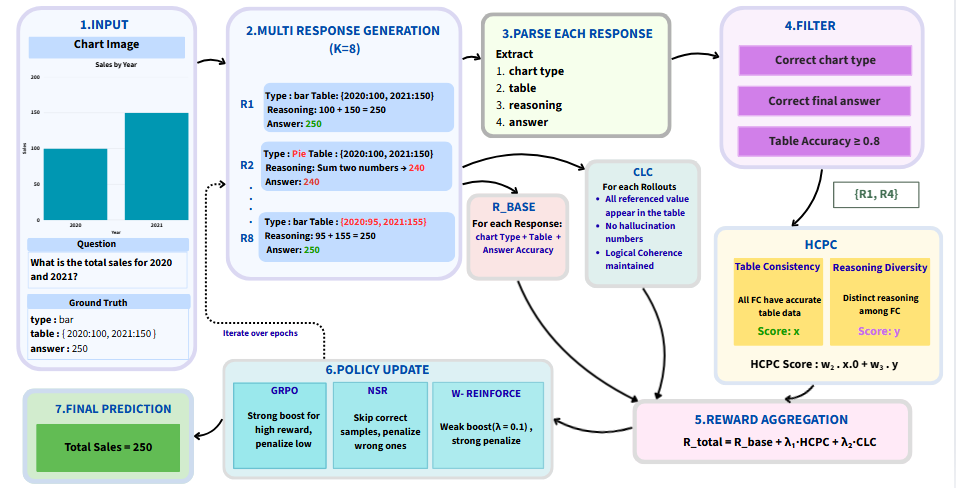
\includegraphics[width=0.85\linewidth]{pipeline.png}
    \caption{Overview of the HCPC-RLVR training pipeline. A chart image and question enter the system; the proposed model generates $K=8$ rollouts; each rollout is parsed into chart type, table, reasoning, and answer; the fully-correct subset feeds HCPC; and the aggregated reward drives the policy update. Current experiments use $K=4$ rollouts because of compute constraints.}
    \label{fig:pipeline}
\end{figure}


\section{Base Model and Parameter-Efficient Fine-Tuning}

The base model is \textbf{Qwen2.5-VL-3B-Instruct}, a 3-billion-parameter vision-language model capable of processing interleaved image and text inputs. Fine-tuning all parameters jointly would be both computationally prohibitive on the available hardware and likely to overfit catastrophically on 1,000 training samples.

Parameter-efficient fine-tuning is applied via Low-Rank Adaptation (LoRA) with rank $r = 8$ and scaling factor $\alpha = 16$, applied to the query and value projection matrices of every attention layer. LoRA inserts two small matrices $A \in \mathbb{R}^{d \times r}$ and $B \in \mathbb{R}^{r \times d}$ in parallel to each targeted weight, computing the effective update as $\Delta W = B A$. This reduces the number of trainable parameters to approximately 4.7 million, which is 0.16\% of the total model size, while all base model weights remain frozen. The low-rank constraint acts as an implicit regularizer limiting the extent to which training on limited data can distort the model's broader visual understanding capabilities. \autoref{fig:lora} illustrates the difference between full-parameter and LoRA fine-tuning.

\begin{figure}[H]
    \centering
    
        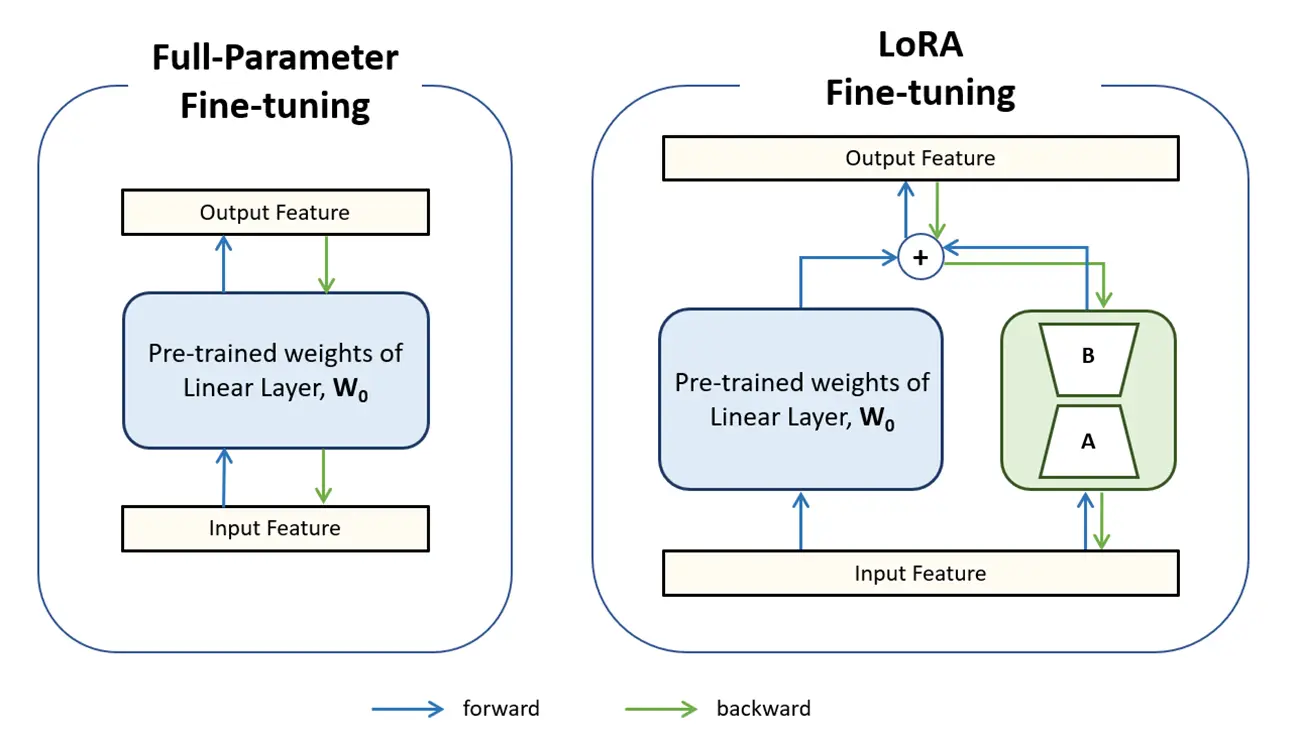
\includegraphics[width=1\linewidth]{lora.png}
      
    \caption{Comparison of full-parameter and LoRA fine-tuning. In LoRA, the adapter matrices are much smaller than the frozen base weights, which keeps the effective parameter count low.}
    \label{fig:lora}
\end{figure}

\section{Structured Output Format and Rollout Generation}

For each chart-question pair, the proposed method generates $K = 8$ candidate responses at temperature 1.0. In the present experiments this was reduced to $K = 4$ to fit the available training and evaluation budget. The model is prompted with a system message that instructs it to think step-by-step and to produce output in the following structured format:

\begin{enumerate}
    \item \texttt{<type>} \textit{chart\_type} \texttt{</type>}: the predicted chart type (bar, line, pie, stacked bar, etc.)
    \item \texttt{<table>} \textit{JSON object} \texttt{</table>}: the extracted data table, with \texttt{"columns"} and \texttt{"rows"} keys
    \item \texttt{<think>} \textit{reasoning steps} \texttt{</think>}: step-by-step chain of thought grounded in the extracted table values
    \item \texttt{<answer>} \textit{final\_answer} \texttt{</answer>}: the final answer to the question
\end{enumerate}

An example of a well-formed response is shown below, for a bar chart comparing satisfaction rates across two years:

\smallskip
\begin{center}
\begin{tabular}{l}
\hline
\texttt{<type> Bar </type>} \\
\texttt{<table> \{"columns": ["Year", "Percentage"], "rows": [["2017", "50"], ["2018", "40"]]\} </table>} \\
\texttt{<think>} \\
\quad \texttt{<step-1>: The question asks for the difference between 2017 and 2018.} \\
\quad \texttt{<step-2>: From the chart: 2017 = 50\%, 2018 = 40\%.} \\
\quad \texttt{<step-3>: Difference = 50\% - 40\% = 10\%.} \\
\quad \texttt{<step-4>: Values verified against extracted table.} \\
\texttt{</think>} \\
\texttt{<answer> 10 </answer>} \\
\hline
\end{tabular}
\end{center}
\smallskip

The structured format serves two purposes. It makes the model's intermediate representations evaluable, allowing reward components to be computed on the extracted table and reasoning trace separately from the final answer. It also enforces a pipeline order --- perception before reasoning before answering --- that mirrors the natural decomposition of the task.

\section{Rollout Count: Intended Design and Current Constraint}

HCPC is a group-level reward, so its quality depends on the number of candidate responses generated for the same chart-question pair. The intended design uses $K=8$ rollouts. With eight responses, table consistency and reasoning diversity can be estimated from a larger set of pairwise comparisons, and the probability of observing at least two fully correct rollouts early in training is higher. This matters because HCPC only fires when the fully correct subset contains at least two rollouts. If too few rollouts are generated, the group-level signal becomes sparse.

The experiments reported in this thesis use $K=4$ because each additional rollout increases both generation cost and memory pressure during GRPO-style training. Under the available Kaggle and local hardware constraints, $K=4$ allowed all variants to complete 2,000 training steps and 500-sample evaluations. The results therefore test whether the HCPC idea is viable under a constrained approximation, not whether the full $K=8$ design has reached its maximum potential. Future experiments should repeat the same protocol with $K=8$ to reduce diversity-estimation noise and to increase the frequency of HCPC reward activation.

\section{Parsing and Filtering}

Each rollout is parsed by extracting the content between its structural tags. A rollout that is missing any tag, or that contains a tag in the wrong order, receives zero reward for the affected component. After parsing, a \emph{fully correct} filter is applied: a rollout is included in the set $R^+$ only if its predicted chart type matches the ground truth, its extracted table passes the table content reward threshold, and its final answer matches the ground truth under the relaxed correctness criterion. This filter prevents lucky guesses --- responses that arrive at the right answer through incorrect extraction or reasoning --- from contaminating the cross-rollout reward computation.

\subsection{Answer Normalization}

Answer matching in chart QA cannot be a strict string comparison. The same numeric answer may appear as \texttt{10}, \texttt{10.0}, \texttt{10\%}, or \texttt{0.10} depending on the unit convention used in the chart and the question. The evaluation therefore applies relaxed matching, following the ChartQA convention, so that small numeric formatting differences do not dominate the measured performance. For categorical answers, normalization removes trivial casing and whitespace differences while preserving the semantic string. This is important for fair comparison: the research question is whether the model reasons correctly from the chart, not whether it exactly reproduces one surface form of a number.

Relaxed matching also has a limitation. It can hide some format-specific failures where the expected answer contains additional qualifiers, such as a party name with a parenthesized score range. For this reason, answer accuracy is interpreted together with format compliance and qualitative error analysis rather than treated as a complete measure of chart reasoning quality.

\subsection{Table Representation}

The extracted table is represented as a JSON object with \texttt{columns} and \texttt{rows}. This representation is simple enough for a language model to generate, but structured enough for automatic parsing and comparison. Table structure reward checks whether the required keys exist and whether the table is syntactically valid. Table content reward compares predicted cell values against the ground truth after normalization. Numeric cells are compared with tolerance; categorical cells are compared after basic text normalization.

The table representation is central to the thesis because it is the bridge between visual perception and reasoning. A model that skips table extraction and answers directly may still be correct on easy examples, but such behavior is difficult to verify and brittle under distribution shift. By making table extraction explicit, the reward can separate perception errors from reasoning errors. HCPC then adds a group-level constraint: correct rollouts should not merely answer correctly, they should agree on the extracted table.

\subsection{Reasoning Step Extraction}

Reasoning diversity is computed from the step-wise reasoning section. The parser extracts step-like units from the \texttt{<think>} block and compares them as sets. Jaccard distance is used as a lightweight approximation of how different two reasoning traces are:
\begin{equation}
    D_{\text{Jaccard}}(S_i, S_j) = 1 - \frac{|S_i \cap S_j|}{|S_i \cup S_j|}
\end{equation}
where $S_i$ and $S_j$ are the reasoning step sets extracted from two rollouts. This metric is intentionally simple and deterministic, but it is not semantically perfect. It may treat paraphrases as different even when they describe the same algorithm, or treat similarly worded steps as identical even when the underlying reasoning differs. The metric is therefore best interpreted as a surface-level diversity proxy, not as a complete semantic measure of reasoning diversity.

\section{Reward Components}

\subsection{Chart-RVR Base Rewards}

The base reward follows the Chart-RVR framework \cite{sinha2025chartrvr} and decomposes into seven components evaluated per rollout:
\begin{equation}
    R_{\text{base}} = \sum_{k=1}^{7} w_k \cdot R_k
\end{equation}
The seven components are: format compliance, chart type prediction, table structure, table content, reasoning quality, final answer correctness, and response length. The format reward verifies that all four tags appear in the correct order. The chart type reward is binary. The table structure reward checks that the JSON has the correct \texttt{"columns"} and \texttt{"rows"} keys. The table content reward numerically compares the extracted values against the ground truth. The reasoning reward evaluates structural quality of the step-by-step trace. The answer reward uses relaxed matching that tolerates minor rounding differences. The length reward penalizes excessively short or long responses.

\subsection{Hierarchical Correct-Path Consistency (HCPC)}

HCPC is a cross-rollout reward computed over the fully correct set $R^+$. Its purpose is to reward the model for being consistently correct across rollouts --- stable table extraction --- while simultaneously rewarding diversity in how the correct rollouts arrive at their answers.

Two sub-scores are computed over $R^+$:
\begin{itemize}
    \item \textbf{Table Consistency} ($C_{\text{table}}$): the average pairwise cosine similarity of the extracted tables across rollouts in $R^+$, measuring how stable the model's visual perception is across multiple generation attempts for the same input.
    \item \textbf{Reasoning Diversity} ($D_{\text{reason}}$): the average pairwise Jaccard distance between the reasoning step sets across rollouts in $R^+$, measuring how different the solution strategies are among correct responses.
\end{itemize}
The HCPC reward combines these with a type consensus term:
\begin{equation}
    R_{\text{HCPC}} = 1.0 \cdot C_{\text{type}} + 2.0 \cdot C_{\text{table}} + 1.5 \cdot D_{\text{reason}}
\end{equation}
The higher weight on $C_{\text{table}}$ (2.0) relative to $D_{\text{reason}}$ (1.5) reflects the priority of extraction stability: inconsistent table extraction directly corrupts downstream reasoning, whereas reasoning diversity is a desirable property rather than a correctness-critical one. HCPC fires only when $|R^+| \geq 2$; if fewer than two rollouts are fully correct for a given training sample, no cross-rollout bonus is applied.

As an example, if two fully correct rollouts extract identical tables ($C_{\text{table}} = 1.0$) and use somewhat different reasoning step sets ($D_{\text{reason}} = 0.67$), the HCPC contribution is:
\begin{equation}
    R_{\text{HCPC}} = 2.0 \times 1.0 + 1.5 \times 0.67 = 2.0 + 1.005 \approx 0.87 \quad (\text{after normalization})
\end{equation}

\subsection{Why HCPC Is Hierarchical}

The term \emph{hierarchical} refers to the dependency structure of chart reasoning. Chart type recognition is a coarse perception decision. Table extraction is a finer perception decision. Reasoning depends on the extracted table, and the final answer depends on both the table and the reasoning. HCPC respects this structure by applying its group-level bonus only after intermediate correctness has been established. The reward is not given merely because multiple rollouts answer correctly. It is given when the correct rollouts form a coherent path from chart type to table to answer.

This design is intended to reduce two failure modes. The first is lucky-answer reinforcement, where the model is rewarded for a correct final answer even though the extracted table is wrong. The second is reasoning collapse, where the model learns a narrow answer template that works on common examples but fails when the chart style or question type changes. By rewarding table agreement and reasoning variation among correct rollouts, HCPC attempts to preserve the parts of the model's behavior that should be stable and the parts that should remain flexible.

\subsection{Correct-Path Filtering}

Correct-path filtering is stricter than answer filtering. A rollout can be answer-correct but excluded from $R^+$ if its chart type or table extraction is wrong. This choice reduces the number of rollouts that contribute to HCPC early in training, but it improves the quality of the group-level signal. Without this filter, HCPC could reward a group of responses that agree on an incorrect table and coincidentally produce the right answer. That would directly undermine the purpose of the method.

The cost of strict filtering is sparsity. When model accuracy is low, many groups have fewer than two fully correct rollouts and therefore receive no HCPC bonus. This is one reason the intended design uses $K=8$: a larger rollout group increases the chance that at least two correct-path responses are present. In the current $K=4$ experiments, the HCPC signal is expected to be weaker than in the full intended setting.

\subsection{Coherence as an Evaluation Signal}

In addition to reward values, the experiments report a coherence metric that estimates reasoning pipeline integrity. Coherence is defined as the probability of a correct answer conditional on a correct table extraction:
\begin{equation}
    \mathrm{Coherence} = P(\text{correct answer} \mid \text{correct table})
\end{equation}
This metric separates perception quality from downstream reasoning quality. A model with high table consistency but low coherence is reading charts consistently but not reasoning reliably from those tables. A model with lower table consistency but higher coherence may fail more often at perception, but reason more faithfully when perception succeeds. Although the updated ChartFC table reports Pass@K as the primary OOD metric, coherence remains useful for diagnosing whether errors originate in extraction or downstream reasoning.

\section{Policy Update Strategies}

\subsection{GRPO}

GRPO computes the advantage for rollout $i$ relative to the group:
\begin{equation}
    \hat{A}_i = R_i - \frac{1}{K} \sum_{j=1}^{K} R_j
\end{equation}
The policy is updated with a KL-penalized objective:
\begin{equation}
    \nabla_\theta J = \sum_{i=1}^{K} \hat{A}_i \cdot \nabla_\theta \log \pi_\theta(\text{response}_i \mid I, Q) - \beta \cdot \mathrm{KL}(\pi_\theta \| \pi_{\text{ref}})
\end{equation}
where $\beta = 0.01$ prevents the trained policy from diverging too far from the reference (initial) model.

\subsection{NSR}

NSR suppresses gradient updates entirely on rollouts deemed correct (reward $\geq \tau$):
\begin{equation}
    \hat{A}_i = \begin{cases} 0 & \text{if } R_i \geq \tau \\ -(1 + R_i) & \text{if } R_i < \tau \end{cases}
\end{equation}
Correct rollouts contribute nothing to the parameter update; incorrect rollouts are penalized in proportion to how wrong they are.

\section{Training Configuration}

All variants share the same base model, LoRA configuration, dataset, and hyperparameters. They differ only in the reward augmentation or advantage computation rule: GRPO uses the base reward, GRPO+HCPC adds the HCPC group-level bonus, and NSR changes the advantage computation so that correct rollouts receive zero gradient while incorrect rollouts are penalized. \autoref{tab:training_config} summarizes the complete training configuration used in the current experiments.

\begin{table}[H]
    \centering
    \begin{tabular}{ll}
        \toprule
        Parameter & Value \\
        \midrule
        Base model & Qwen2.5-VL-3B-Instruct \\
        Fine-tuning method & LoRA ($r=8$, $\alpha=16$, q\_proj + v\_proj) \\
        Trainable parameters & $\sim$4.7M (0.16\% of total) \\
        Optimizer & AdamW \\
        Learning rate & $1 \times 10^{-5}$ \\
        Rollouts per sample ($K$) & 4 in current experiments; 8 in intended HCPC design \\
        Training temperature & 1.0 \\
        Training steps & 2,000 \\
        Precision & bf16 mixed \\
        Effective batch size & 4 (2 per device $\times$ 2 accumulation steps) \\
        KL penalty ($\beta$) & 0.01 \\
        HCPC weights & $w_{\text{type}}=1.0$,\ $w_{\text{table}}=2.0$,\ $w_{\text{reason}}=1.5$ \\
        HCPC scaling $\lambda$ & 1.0 \\
        \bottomrule
    \end{tabular}
    \caption{Training configuration shared across all HCPC-RLVR variants}
    \label{tab:training_config}
\end{table}


\chapter{Results and Discussion} \label{chapter:results}

\section{Experimental Setup}

\subsection{Hardware and Software Environment}

Training was performed on Kaggle, with an NVIDIA H100 40GB GPU used as the primary training environment in the project setup. Evaluation, debugging, and inference were run on a local machine with an NVIDIA RTX 3090 24GB GPU. The software environment used the \texttt{transformers} and \texttt{trl} libraries for model loading and the GRPO training loop, \texttt{peft} for LoRA adapter integration, \texttt{bitsandbytes} for bf16 mixed-precision training, and \texttt{vllm} for fast batch inference during evaluation. Under the current $K=4$ constrained setting, each method required roughly six hours for 2,000 training steps.

\subsection{Training Dataset}

The training data are drawn from the Chart-RVR GRPO Train dataset \cite{sinha2025chartrvr}, which contains 34,194 samples sourced from ChartQA, PlotQA, and ChartFC. Each enriched sample includes a chart image, a chart type label, a ground-truth data table, a reasoning chain, and a final answer. Compute constraints limited us to the first 1,000 samples using \texttt{dataset.select(range(1000))}, without shuffling. The distribution of chart types in this subset is shown in \autoref{tab:training_data}.

\begin{table}[H]
    \centering
    \begin{tabular}{lrr}
        \toprule
        Chart Type & Count & Proportion \\
        \midrule
        Bar         & 485 & 48.5\% \\
        Line        & 223 & 22.3\% \\
        Stacked Bar & 147 & 14.7\% \\
        Pie         & 145 & 14.5\% \\
        \midrule
        \textbf{Total} & \textbf{1,000} & \textbf{100\%} \\
        \bottomrule
    \end{tabular}
    \caption{Chart type distribution in the 1,000-sample training subset}
    \label{tab:training_data}
\end{table}

Bar charts make up nearly half the training subset, and together with line charts account for over 70\%. Scatterplot and bubble chart samples are absent from this subset. This imbalance has direct consequences for per-chart-type performance discussed later in this chapter.

The subset differs from the full Chart-RVR training set in two important ways. First, the first 1,000 samples are more concentrated in bar and line charts than the full set. Second, the subset has a higher proportion of numerical labels than the full corpus. This matters because numeric chart QA questions place more pressure on value extraction and arithmetic, while categorical questions place more pressure on label grounding and answer formatting. The current results should therefore be read as performance on a value-extraction-heavy subset rather than a balanced estimate over all chart types.

\begin{table}[H]
    \centering
    \small
    \begin{tabular}{lrrrrr}
        \toprule
        Chart Type & Full Count & Full Prop. & 1K Count & 1K Prop. & 1K Numerical Labels \\
        \midrule
        Bar & 13,682 & 40.0\% & 485 & 48.5\% & 69.5\% \\
        Line & 3,682 & 10.8\% & 223 & 22.3\% & 64.6\% \\
        Stacked Bar & 2,740 & 8.0\% & 147 & 14.7\% & 72.1\% \\
        Pie & 2,136 & 6.2\% & 145 & 14.5\% & 62.1\% \\
        Scatterplot & 540 & 1.6\% & 0 & 0.0\% & -- \\
        Bubble & 8 & 0.0\% & 0 & 0.0\% & -- \\
        No annotation & 11,398 & 33.3\% & 0 & 0.0\% & -- \\
        \bottomrule
    \end{tabular}
    \caption{Comparison between the full Chart-RVR training set and the first 1,000-sample subset used in this thesis}
    \label{tab:full_vs_subset}
\end{table}

\subsection{Evaluation Benchmark and Protocol}

The primary in-distribution evaluation benchmark is the 500-sample Chart-RVR GRPO Test 151 split, drawn from ChartQA and PlotQA-style chart QA samples. All four methods --- Base (untrained), GRPO, GRPO+HCPC, and NSR --- are evaluated on the same samples. For each test sample, the model generates 4 responses at temperature 0.8 and top-$p$ 0.95. The evaluation metrics are summarized in \autoref{tab:metrics}.

For continuity with the earlier ChartQA-only analysis, \autoref{tab:chartqa_eval_distribution} reports the chart-type distribution of the 500-sample ChartQA subset used during predefense preparation. The updated headline results use the Chart-RVR GRPO Test 151 split, but the same qualitative difficulty patterns remain relevant: short answers should not be confused with easy reasoning, because many questions require multi-step computation or decimal precision.

\begin{table}[H]
    \centering
    \begin{tabular}{lrr}
        \toprule
        Chart Type & Count & Proportion \\
        \midrule
        Bar & 316 & 63.2\% \\
        Line & 142 & 28.4\% \\
        Pie & 41 & 8.2\% \\
        Scatterplot & 1 & 0.2\% \\
        \bottomrule
    \end{tabular}
    \caption{Chart type distribution in the earlier 500-sample ChartQA evaluation subset}
    \label{tab:chartqa_eval_distribution}
\end{table}

\begin{table}[H]
    \centering
    \begin{tabular}{lp{1.8cm}p{7cm}}
        \toprule
        Metric & Range & Definition \\
        \midrule
        Accuracy (Acc\%) & 0--100\% & Fraction of samples where at least one rollout is correct (relaxed match) \\
        Pass@$K$ & 0--100\% & Probability that at least 1 of $K$ responses is correct \cite{chen2021evaluating} \\
        $C_{\text{table}}$ & 0.0--1.0 & Cosine similarity of extracted tables across rollouts --- perception stability \\
        $D_{\text{reason}}$ & 0.0--1.0 & Jaccard distance of reasoning step sets across rollouts --- strategy diversity \\
        Coherence & 0.0--1.0 & Probability of a correct answer given a correct table extraction \\
        Format\% & 0--100\% & Fraction of responses with all required structural tags in the correct order \\
        \bottomrule
    \end{tabular}
    \caption{Evaluation metrics and their definitions}
    \label{tab:metrics}
\end{table}

The final evaluation tables report Pass@K as the primary inference-scaling metric. A sample counts as solved if at least one of the first $K$ sampled responses is correct. This is especially appropriate for rollout-based RLVR because it captures whether training improves the probability of obtaining a correct answer when several stochastic responses are available.

\section{Main Results}

\autoref{tab:main_results} reports the updated evaluation results from the 500-sample Chart-RVR GRPO Test 151 split, which contains ChartQA and PlotQA samples. All trained variants outperform the base model across Pass@K.

\begin{table}[H]
    \centering
    \small
    \begin{tabular}{lrrr}
        \toprule
        Method & Pass@1 & Pass@2 & Pass@4 \\
        \midrule
        Base (no training) & 59.45 & 74.33 & 84.46 \\
        GRPO & 73.0 & 82.2 & 87.31 \\
        GRPO+HCPC (ours) & 72.85 & \textbf{84.57} & \textbf{88.70} \\
        NSR (ours --- first VLM) & \textbf{73.4} & 83.72 & 88.00 \\
        \bottomrule
    \end{tabular}
    \caption{Performance evaluation on Chart-RVR GRPO Test 151 (ChartQA and PlotQA, 500 samples). Bold indicates the best value per column.}
    \label{tab:main_results}
\end{table}

\section{Analysis}

\subsection{RLVR Provides Consistent Improvement Over the Baseline}

Every RLVR-trained variant improves meaningfully over the untrained base model. Pass@1 rises from 59.45\% for the base model to 73.0\% for GRPO, 72.85\% for GRPO+HCPC, and 73.4\% for NSR. Pass@4 also improves from 84.46\% to 87.31\%, 88.70\%, and 88.00\%, respectively. This directly answers the first research question: RLVR with 1,000 training samples and a 3B-parameter model is sufficient to produce meaningful improvements in chart QA rollout accuracy under the current resource-constrained setting.

\subsection{HCPC Improves Rollout-Level Reliability}

GRPO+HCPC achieves the highest Pass@2 (84.57\%) and highest Pass@4 (88.70\%). The Pass@K comparison is particularly informative: GRPO+HCPC is 2.37 percentage points above GRPO at Pass@2 (84.57\% vs.\ 82.2\%) and 1.39 percentage points above GRPO at Pass@4 (88.70\% vs.\ 87.31\%). NSR has a slightly higher Pass@1 than HCPC (73.4\% vs.\ 72.85\%), but HCPC retains the strongest multi-rollout behavior at Pass@2 and Pass@4.

This answers the second research question with a more specific pattern: HCPC, by conditioning the training bonus on intermediate step correctness, improves over flat GRPO rewards most clearly when multiple rollouts are available.

\subsection{NSR Transfers Successfully to Vision-Language Models}

NSR achieves the best Pass@1 score (73.4\%) and an 88.00\% Pass@4, placing it close to GRPO+HCPC and clearly above the base model. This answers the third research question affirmatively: NSR, originally designed for text-based mathematics, transfers successfully to a vision-language model with noisy, multi-component rewards. The first VLM application of NSR is competitive with HCPC and substantially stronger than the untrained baseline on this updated evaluation.

\subsection{HCPC vs.\ NSR: Explicit vs.\ Implicit Diversity Promotion}

GRPO+HCPC and NSR produce similar but not identical Pass@K profiles. NSR has the edge at Pass@1 (73.4\% vs.\ 72.85\%), while HCPC has the edge at Pass@2 (84.57\% vs.\ 83.72\%) and Pass@4 (88.70\% vs.\ 88.00\%). This suggests that explicit correct-path reward shaping and implicit negative-only diversity preservation are complementary: NSR is slightly stronger when only one rollout is used, while HCPC is stronger when multiple sampled reasoning paths are available.

This answers the fourth research question: explicit diversity engineering via HCPC and implicit diversity preservation via NSR are broadly competitive, with HCPC leading the in-distribution multi-rollout metrics and NSR remaining the strongest single-rollout alternative.

\subsection{Per-Chart-Type Analysis}

Earlier per-chart-type analysis reveals a pattern obscured in the aggregate numbers. Bar-chart questions benefit most clearly from HCPC-style hierarchical extraction rewards, while line-chart questions show weaker gains because they often require temporal or trend reasoning rather than direct value comparison. Pie-chart comparisons are less stable because the sample count is small.

The line chart result is a notable finding. Line chart questions frequently require temporal or trend reasoning --- identifying when a value first crossed a threshold, comparing rates of change across intervals --- rather than simple value extraction. None of the current reward components specifically reward trend reasoning, which means the reward design has an implicit bias toward value-extraction tasks aligned with bar chart structure. Extending the reward design to include components that target trend reasoning would be necessary to avoid this degradation.

\subsection{Reasoning Diversity}

All methods show low $D_{\text{reason}}$ values in the range 0.04--0.058. The absolute differences between methods are small. Two factors likely contribute to this. First, $K=4$ evaluation rollouts may be insufficient to reliably estimate Jaccard diversity over reasoning step sets; the HCPC diversity incentive was designed for $K=8$ and may require higher $K$ at evaluation to observe its full effect. Second, HCPC does not directly penalize lexically similar reasoning chains; it only rewards diversity among correct rollouts, which is a positive incentive rather than a hard diversity constraint.

\subsection{Pass@4 Rollout Reliability}

Pass@4 answers the question: ``does at least one of the four sampled responses solve the problem?'' It is especially relevant for chart QA because multiple stochastic rollouts can expose whether a method maintains several viable routes to the same answer.

The updated Pass@4 results provide the strongest current evidence for HCPC's rollout reliability benefit. GRPO+HCPC reaches 88.70\% Pass@4, compared with 87.31\% for GRPO and 88.00\% for NSR. The method does not simply increase single-rollout correctness; it increases the probability that at least one of several sampled reasoning paths reaches the correct answer. This aligns with the design of HCPC: among correct rollouts, reward stable extraction and controlled reasoning variation so that the model becomes more reliable across repeated generations.

\subsection{Format Compliance}

The structured-output format remains practically important even though the updated headline results emphasize Pass@K. The reward computation depends on parseable \texttt{<type>}, \texttt{<table>}, \texttt{<think>}, and \texttt{<answer>} sections. A model that answers correctly but omits tags cannot be evaluated reliably by the training loop, so format validity remains a necessary condition for trustworthy reward computation.

\subsection{Result Distribution}

The per-sample reward distribution is bimodal for all trained methods. Samples tend to cluster near zero, where the model repeatedly fails, or near one, where the model solves the sample reliably. Intermediate scores are rare. This suggests that RLVR does not primarily create many partially correct responses. Instead, it moves samples from an unsolved region to a solved region. GRPO+HCPC shifts mass rightward relative to the base model, and NSR shows the strongest OOD transfer in the updated ChartFC experiments.

This pattern has two implications. First, Pass@K gains may understate some behavioral improvement because they do not show how many correct rollouts a solved sample contains. A method that changes many samples from one-correct-rollout behavior to multi-correct-rollout behavior improves reliability even when a binary solved/not-solved metric changes only modestly. Second, the hard sample set is meaningful. Samples that remain near zero after all training variants likely require capabilities not supplied by the current reward design, such as high-precision visual reading, color grounding, or symbolic computation.

\section{Out-of-Distribution Evaluation on ChartFC}

The updated predefense experiments include an out-of-distribution comparison on ChartFC for GRPO, GRPO+HCPC, and NSR. ChartFC differs from ChartQA because it is framed as chart-based fact checking rather than open-ended question answering. The model must decide whether a claim is supported, refuted, or insufficiently grounded by the chart. This changes both the input distribution and the reasoning objective, making it a useful diagnostic of whether the trained reward strategy transfers beyond the immediate ChartQA setting.

\begin{table}[H]
    \centering
    \small
    \begin{tabular}{lrrr}
        \toprule
        Method & Pass@1 & Pass@2 & Pass@4 \\
        \midrule
        GRPO & 62.45 & 79.9 & 81.8 \\
        GRPO+HCPC & 61.22 & 80.1 & 83.14 \\
        NSR & \textbf{68.70} & \textbf{82.60} & \textbf{92.40} \\
        \bottomrule
    \end{tabular}
    \caption{Out-of-distribution evaluation on ChartFC (500 samples). Bold indicates the best value per column.}
    \label{tab:chartfc_results}
\end{table}

The ChartFC results show NSR as the strongest OOD method across all reported Pass@K metrics. GRPO obtains 62.45\% Pass@1 and 81.8\% Pass@4. GRPO+HCPC is slightly lower than GRPO at Pass@1 (61.22\% vs.\ 62.45\%), but improves the multi-rollout metrics to 80.1\% Pass@2 and 83.14\% Pass@4. NSR achieves the strongest OOD transfer, with 68.70\% Pass@1, 82.60\% Pass@2, and 92.40\% Pass@4. The result supports the hypothesis that diversity-preserving reward design is especially valuable under distribution shift: NSR's negative-only update rule provides the strongest OOD robustness among the evaluated methods.

This updated OOD result changes the interpretation of the method comparison. Earlier analysis treated HCPC's main OOD advantage as conditional coherence. The current results show a stronger top-line finding: NSR is the best-performing method on all reported ChartFC metrics, while HCPC mainly improves over GRPO when more than one rollout is available. This makes NSR a stronger candidate for future combination with HCPC, because it already preserves generalizable behavior under distribution shift while HCPC provides explicit correct-path consistency.

\section{Sample Difficulty Analysis}

The 500 ChartQA samples can be divided into three broad categories. The first category contains samples solved by all four methods, including the base model. These are visually clear charts with straightforward questions, and they account for 344 samples (68.8\%). The second category contains samples solved by some trained methods but not all methods. These 82 samples (16.4\%) are the most informative for comparing reward strategies because training changes the outcome. The third category contains samples solved by no method. These 52 samples (10.4\%) represent the current capability ceiling of the 3B model and reward design.

\begin{table}[H]
    \centering
    \begin{tabular}{lrr}
        \toprule
        Difficulty category & Count & Proportion \\
        \midrule
        Solved by all four methods & 344 & 68.8\% \\
        Solved by some trained methods only & 82 & 16.4\% \\
        Solved by no method & 52 & 10.4\% \\
        Remaining mixed/parse-dependent cases & 22 & 4.4\% \\
        \bottomrule
    \end{tabular}
    \caption{ChartQA sample difficulty categories from the predefense analysis}
    \label{tab:difficulty_categories}
\end{table}

The contested 82 samples are where reward design matters most. Each trained method uniquely solves a small number of samples that the others miss, while pairwise Jaccard similarity among trained methods remains high (approximately 0.864--0.881). This means the methods are complementary, but not orthogonal. They mostly improve the same region of the task distribution, with modest differences in which borderline cases they solve.

\section{Hard Problem Types}

Manual inspection of the lowest-scoring examples reveals several recurring failure modes. Decimal precision questions are particularly difficult. In one example, the correct answer is 3.0238, but models consistently answer 3.0 or 3.02. The models identify the correct bar but cannot read sub-hundredth precision from the chart image. This is a perception limitation, not a reasoning limitation.

Cross-element arithmetic is another common failure mode. Ratio and difference questions require two or more extracted values, followed by arithmetic. A small error in either extraction is amplified by the computation. Color and legend grounding also causes failures, especially in multi-line charts where the question refers to a line by semantic category and the answer requires a color such as ``green line.'' The current reward components do not explicitly reward color-category binding.

\begin{table}[H]
    \centering
    \begin{tabular}{p{3.4cm}p{3cm}p{5.3cm}}
        \toprule
        Problem type & Example answer & Why it fails \\
        \midrule
        Decimal precision & 3.0238 & Axis resolution is insufficient; the model rounds visually read values \\
        Cross-element arithmetic & 1.217 & Extraction errors compound through division or subtraction \\
        Color/label grounding & green line & The model must bind a visual color to a semantic legend category \\
        Sub-percent difference & 0.03 & The difference is visually indistinguishable at image resolution \\
        Exact format match & Democrat (scores 60 to 100) & The model may know the content but miss the exact expected string format \\
        Non-chart reasoning & 4.1 & The input resembles a number-pattern problem more than chart reasoning \\
        \bottomrule
    \end{tabular}
    \caption{Common hard problem types observed in low-scoring samples}
    \label{tab:hard_problem_types}
\end{table}

These failures clarify what the current method does and does not solve. HCPC can improve reliability when the model has enough visual information to extract the table and enough prior ability to reason over it. It cannot recover values that are visually unreadable at the input resolution, and it does not by itself add symbolic tools for exact arithmetic. This motivates future work on program-of-thought execution, higher-resolution chart parsing, and color-aware visual grounding rewards.

\section{Why Diversity Did Not Improve Strongly}

One expected outcome of HCPC is higher reasoning diversity, because the reward contains a $D_{\text{reason}}$ term. The observed ChartQA results do not show a strong diversity improvement: GRPO has $D_{\text{reason}}=0.058$, HCPC has 0.052, and NSR has 0.057. This does not invalidate the HCPC idea, but it does show that the current implementation and resource setting are not sufficient to demonstrate that part of the design conclusively.

There are four likely causes. First, the current experiments use $K=4$, while the intended design uses $K=8$. Diversity over four responses is a noisy estimate, especially when only a subset of the responses are fully correct. Second, HCPC only fires when at least two rollouts are fully correct, so early in training the diversity signal may be sparse. Third, the table consistency weight (2.0) is higher than the reasoning diversity weight (1.5), which intentionally prioritizes stable perception but may cause consistency to dominate the group reward. Fourth, Jaccard distance over extracted reasoning step sets is a coarse metric. Two reasoning chains may be semantically different but lexically similar, or lexically different but algorithmically identical.

The interpretation is therefore conservative: HCPC shows clear rollout reliability benefits under $K=4$, but the diversity component needs the full $K=8$ setting and possibly a stronger semantic diversity metric before it can be judged fairly.

\section{Limitations}

The training subset of 1,000 samples is too small to produce statistically significant differences between methods at the performance levels observed. Bootstrap confidence intervals for method pairs overlap substantially in earlier analysis, and the observed gaps should be interpreted as directional evidence rather than definitive rankings. Training on the full 34,194-sample dataset would be necessary to draw firm conclusions.

The evaluation covers one in-distribution test split and one out-of-distribution benchmark, ChartFC. Broader OOD performance on EvoChart, ChartBench, and ChartQAPro is still needed to establish whether the learned reward conditioning generalizes beyond the current setting. The available evidence suggests that NSR is strongest on the current ChartFC transfer task, while GRPO+HCPC is strongest on the in-distribution Pass@2 and Pass@4 metrics.

All experiments use a single 3B-parameter model. Whether the HCPC vs.\ NSR dynamics observed here hold at larger model scales (7B, 72B) is unknown and is the most important open question for follow-up work.

\section{Threats to Validity}

\subsection{Internal Validity}

The main internal validity risk is that the current experiments do not run the full intended $K=8$ rollout setting. HCPC is explicitly designed around group-level statistics, and these statistics are less reliable when estimated from four responses. A weaker diversity signal under $K=4$ may make HCPC appear less effective at promoting reasoning diversity than it would be under the full design. The results therefore support the viability of HCPC, but not the final magnitude of its intended effect.

A second internal validity risk is parser dependence. Format compliance is high for trained models, but any reward framework that relies on structural tags can mis-score responses when tags are malformed or nested unexpectedly. This risk is partially mitigated by reporting format compliance separately, but parser behavior can still influence reward values during training.

\subsection{External Validity}

The 1,000-sample training subset is not a balanced sample of all chart types. It contains no scatterplots or bubble charts and is heavily weighted toward bar and line charts. As a result, the conclusions are strongest for the chart types represented in training and weaker for rare chart families. The ChartFC OOD experiment provides useful evidence that reward effects transfer differently across distributions, and the updated evaluation now includes GRPO, GRPO+HCPC, and NSR. A complete external validity claim would still require evaluating all methods on additional OOD benchmarks such as EvoChart, ChartBench, and ChartQAPro.

\subsection{Construct Validity}

The metrics used in this thesis measure useful but incomplete constructs. $C_{\text{table}}$ measures consistency of extracted tables, but high consistency can mean consistently correct extraction or consistently repeated errors unless interpreted alongside accuracy. $D_{\text{reason}}$ measures surface-level diversity of reasoning steps, but not necessarily semantic diversity. Coherence measures whether correct tables lead to correct answers, but it does not capture whether the written reasoning explanation is human-faithful. These limitations are why the analysis combines quantitative metrics with qualitative hard-case inspection.

\subsection{Statistical Conclusion Validity}

The observed differences between methods are modest in some settings, and the 500-sample evaluation size limits statistical power. The predefense analysis notes that statistical significance is not reached at the current scale. Therefore, claims in this thesis are framed as directional and diagnostic. The strongest conclusions are those supported by consistent patterns across related metrics, such as HCPC's in-distribution rollout reliability improvement and NSR's stronger ChartFC OOD transfer.


\chapter{Conclusion} \label{chapter:conclusion}

\section{Summary of What We Did}

This thesis proposed HCPC-RLVR, a reinforcement learning framework for chart question answering with an original reward-design contribution beyond standard GRPO training. The Hierarchical Correct-Path Consistency reward conditions a cross-rollout bonus on intermediate step correctness, rewarding consistent table extraction and diverse reasoning among fully-correct rollouts simultaneously. Negative Sample Reward was applied to a vision-language model for the first time, extending Zhu et al.'s negative-only reinforcement mechanism from text-based mathematics to a multi-modal setting with noisy, multi-component rewards.

All methods were trained on Qwen2.5-VL-3B-Instruct with LoRA on 1,000 samples and evaluated on 500 in-distribution Chart-RVR GRPO Test 151 samples and 500 out-of-distribution ChartFC samples. The intended HCPC design uses $K=8$ rollouts; the present experiments use $K=4$ because of resource constraints. The central comparison between HCPC (explicit diversity engineering) and NSR (implicit diversity preservation) found both to be strong, with complementary strengths: GRPO+HCPC leads the in-distribution Pass@2 and Pass@4 metrics, while NSR leads in-distribution Pass@1 and the ChartFC out-of-distribution metrics.

\section{Summary of Results}

\begin{table}[H]
    \centering
    \begin{tabular}{ll}
        \toprule
        Finding & Result \\
        \midrule
        RLVR improves over base model & Pass@1: 59.45\% $\rightarrow$ 72.85--73.4\% \\
        GRPO+HCPC best in-distribution Pass@2 & \textbf{84.57\%} vs.\ 82.2\% for GRPO \\
        GRPO+HCPC best in-distribution Pass@4 & \textbf{88.70\%} vs.\ 87.31\% for GRPO \\
        NSR best in-distribution Pass@1 & \textbf{73.4\%} vs.\ 72.85\% for GRPO+HCPC \\
        NSR best ChartFC OOD Pass@1 & \textbf{68.70\%} vs.\ 61.22\% for GRPO+HCPC \\
        NSR best ChartFC OOD Pass@4 & \textbf{92.40\%} vs.\ 83.14\% for GRPO+HCPC \\
        \bottomrule
    \end{tabular}
    \caption{Summary of key findings}
    \label{tab:summary}
\end{table}

\section{Limitations}

The 1,000-sample training subset is insufficient for statistically significant conclusions; observed differences between methods are directional. All experiments use a single 3B-parameter model. The current experiments use $K=4$ rather than the intended $K=8$, making reasoning-diversity estimates noisy and likely underestimating HCPC's group-level effect. The updated ChartFC evaluation now includes GRPO, GRPO+HCPC, and NSR, but broader OOD evaluation on EvoChart, ChartBench, and ChartQAPro is still needed before making general claims about distribution-shift robustness.

\section{Future Work}

\textbf{Complete $K=8$ experiments.} The proposed HCPC method is designed for eight rollouts per sample. Repeating training and evaluation with $K=8$ would provide a cleaner estimate of table consistency and reasoning diversity, and would increase the number of groups where at least two correct rollouts exist for HCPC reward computation.

\textbf{Model scale and full training.} Extending to 7B- and 72B-parameter models and training on the full 34,194-sample Chart-RVR dataset would establish whether the HCPC and NSR dynamics persist at scale and whether statistically significant accuracy margins emerge.

\textbf{Entropy-based diversity.} The Jaccard-distance-based $D_{\text{reason}}$ metric is a coarse proxy for reasoning diversity that depends on surface-level textual similarity between step descriptions. Directly regularizing the entropy of the rollout distribution during training would provide explicit, continuous control over diversity without this dependence.

\textbf{Trend and temporal reasoning rewards.} Adding reward components specifically targeting line chart reasoning --- correct identification of monotonic periods, rate-of-change comparisons, and threshold-crossing detection --- would address the observed degradation on line chart questions and reduce the current reward design's implicit bar chart bias.

\textbf{Out-of-distribution robustness.} Systematic evaluation on ChartFC, EvoChart, and ChartBench would characterize the generalization boundaries of each reward strategy and identify whether domain-adaptive training is needed for out-of-distribution chart distributions.

\section{Concluding Remarks}

The results of this thesis demonstrate that reward design, not just model capacity, is a meaningful lever for improving structured visual reasoning in chart question answering. Even at 3 billion parameters and 1,000 training samples, RLVR training produces consistent and substantial gains over an untrained model. HCPC's cross-rollout conditioning on intermediate correctness and NSR's implicit diversity preservation through negative-only reinforcement represent two distinct and compatible approaches to the problem of reasoning collapse --- one that explicitly engineers what the model should do, and one that removes the pressure causing it to overfit. Understanding which approach is preferable at larger scales and on more diverse chart distributions is the most important direction for future work.

%-------------------------- BACK MATTER --------------------------%

\printbib

\end{document}
